\documentclass[11pt,a4paper]{report}
\usepackage[utf8]{inputenc}
\usepackage[french]{babel}
\usepackage[T1]{fontenc}
\usepackage{amsmath}
\usepackage{amsfonts}
\usepackage{amssymb}
\usepackage[left=2cm,right=2cm,top=2cm,bottom=2cm]{geometry}
\usepackage{graphicx}

\begin{document}
\tableofcontents
\chapter{Le phénomène de diffraction}
	\section{Rappels théorique}
\paragraph{}	
Le phénomène de diffraction que nous étudions apparait lorsqu'une onde passe à travers une fente d'une largeur inférieure à sa longueur d'onde $\lambda$. Il en résulte une modification de la propagation de cette onde  au-delà de l'obstacle : pour une onde plane, les fronts d'onde obtenus sont presque circulaires.
\paragraph{}
Afin d'observer ce phénomène, nous réalisons une expérience qui consiste à faire passer
un rayon monochromatique de longueur d'onde $\lambda$ au travers une fente très mince de largeur b, et à projeter ce rayon sur un écran situé à une distance D de l'obstacle. 
\paragraph{}
D'après la théorie, les fronts d'onde du rayon diffracté étant circulaires, nous devrions donc observer sur l'écran une succession de franges sombres et de franges lumineuses dont l'intensité maximale et la taille varient selon la position sur l'écran.
Cet ensemble de franges forme une figure de diffraction symétrique dont l'intensité est proportionnelle au carré de l'amplitude de l'onde et dépend de l'angle $\theta$ :
\paragraph{}
\begin{equation}
I_{\theta} = I_{0} \frac{sin^{2}\beta}{•\beta^{2}}
\end{equation}
\begin{equation}
\beta = \frac{\pi.b.sin\theta}{\lambda}
\end{equation}
\begin{equation}
\sin\theta \approx \tan\theta = \frac{z}{D}
\end{equation}
\paragraph{}
\subparagraph{•}
Les minima apparaissent pour $\beta = \pi,2\pi...$
\subparagraph{•}
Les maxima  sont obtenus pour $\beta = 1,43\pi...$
\paragraph{}
L'expérience est réalisée en utilisant dans un premier temps une fente rectangulaire et ensuite une fente circulaire.


	\section{Schéma de principe}
	voir figure \ref{schemadeprincipe} p.\pageref{schemadeprincipe}
	\begin{figure}[!]
	\caption{\label{schemadeprincipe} Schéma de principe de l'expérience}
	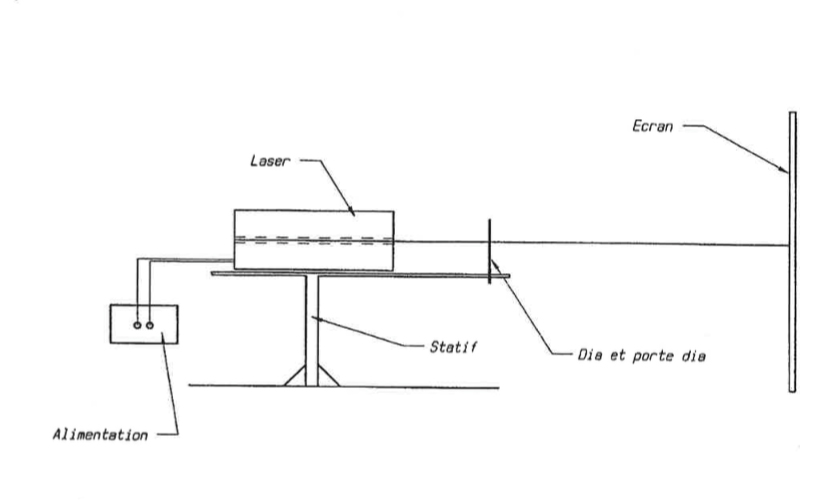
\includegraphics[scale=0.5]{schemadeprincipe.jpg}
	\end{figure}
	\section{Liste du matériel}
	\begin{itemize}
	\item laser monochromatique
	\item mètre ruban
	\item dias à fente rectangulaire
	\item dias à fente circulaire
	\item porte dia
	\item écran de projection
	\item statif
	\end{itemize}
	\section{Principe de l'expérience}
	La manipulation consiste à vérifier la figure de diffraction obtenue et à mesurer la position des minima d'intensité observés sur l'écran pour en déduire la longueur d'onde du rayon projeté, ceci grâce à la relation  
	$\lambda = \frac{\pi.e.z}{\beta.D}$. Nous pouvons alors comparer cette valeur avec la valeur théorique de $\lambda$ qui est connue pour le laser utilisé.
	\section{Tableau de mesures}
	\subsection{Expérience avec fente rectangulaire}
	\begin{center}	
	\begin{tabular}{|c|c|c|c|c|c|c|}
		\hline
		\bf n & \bf D & \bf $\Delta$D & \bf z & \bf $\Delta$z & \bf $\lambda$& \bf $\Delta\lambda$ \\
		\hline
		 & \bf [mm] & \bf [mm] & \bf [mm] & \bf [mm] & \bf [nm]  & \bf [nm] \\
		\hline
		4 & 5670 & 50 & 118 &  1 & 772 &  13\\
		5 & 5670 & 50 & 146 &  1 & 618 &  9\\
		\hline
	\end{tabular}
	\end{center}
	\subsection{Expérience avec fente circulaire}
	\begin{center}
	
	\begin{tabular}{|c|c|c|c|c|c|c|}
		\hline
		\bf n & \bf D & \bf $\Delta$D & \bf z & \bf $\Delta$z & \bf $\oslash$& \bf $\Delta\oslash$ \\
		\hline
		 & \bf [mm] & \bf [mm] & \bf [mm] & \bf [mm] & \bf [mm]  & \bf [mm] \\
		\hline
		4 & 5670 & 50 & 34&  1 &0,41 & 0,02 \\
		5 & 5670 & 50 & 42&  1 &0,42 & 0,02\\
		\hline
	\end{tabular}
	\end{center}	
	\section{Calculs}
		\subsection{Expérience avec fente rectangulaire}
		\subsubsection{Calcul de la longueur d'onde $\lambda$ du rayon laser}
		\begin{equation}
		\lambda = \frac{a.z_{n}}{n.D}		
		\end{equation}		 
		où
		 \begin{itemize}
		  \item a est la largeur de la fente
		  \item D est la distance écran-dia
		  \item n est ordre
		  \item z est distance du minima 
		 \end{itemize}
		\subsubsection{Calcul de l'incertitude de $\lambda$}
		\begin{equation}
		\frac{\Delta \lambda}{\lambda} = \frac{\Delta\left(\frac{a.z_{n}}{n.D}\right)}{\frac{a.z_{n}}{n.D}} 
		= \frac{\Delta D}{D}+\frac{\Delta z_{n}}{z_{n}}
		\end{equation}
		\begin{equation}
		\Delta \lambda
		= \left(\frac{\Delta D}{D}+\frac{\Delta z_{n}}{z_{n}}\right).\lambda
		\end{equation}
		\begin{center}
		$\Delta \lambda = \left(\frac{50}{5670}+\frac{1}{118}\right) 618 = 9 nm$
		\end{center}
		\subsection{Expérience avec fente circulaire}
		\subsubsection{Calcul de la longueur du diamètre de la fente}
		\begin{equation}
		a = \frac{\lambda.n.D}{z_{n}}
		\end{equation}
		\begin{center}
		$a = \frac{618.10^{-6}.4.5670}{42} = 0,4 mm$
		\end{center}
		\subsubsection{Calcul de l'incertitude sur le diamètre de la fente}
		\begin{equation}
		\frac{\Delta a}{a} =\frac{\Delta\left(\frac{\lambda.n.D}{z_{n}}\right)}{ \frac{\lambda.n.D}{z_{n}}} = \frac{\Delta D}{D}+\frac{\Delta z_{n}}{z_{n}}+ \frac{\Delta \lambda}{\lambda}
		\end{equation}
		\begin{equation}
		\Delta a = \left(\frac{\Delta D}{D}+\frac{\Delta z_{n}}{z_{n}}+\frac{\Delta \lambda}{\lambda}\right).a
		\end{equation}
		\begin{center}
		$\Delta a = \left(\frac{50}{5670}+\frac{1}{118}+\frac{9}{618}\right).0,41 = 0,02 mm$
		\end{center}
	\section{Conclusion}
\chapter{Le phénomène d'interférence}
	\section{Rappels théorique}
\paragraph{}	
Le phénomène d'interférence a lieu lorsque deux ondes se rencontrent et se chevauchent pour produire des points d'interférence constructive ou destructive.
\paragraph{}
Pour observer ce phénomène, nous faisons passer un rayon monochromatique de longueur d'onde $\lambda$ au travers de deux fentes minces espacées d'une longueur d, de manière à engendrer deux sources ponctuelles cohérentes. Nous plaçons un écran face à l'obstacle et à une distance D de celui-ci de manière à obtenir la figure d'interférence des ondes. 
\paragraph{}
Si nous pouvions isoler le phénomène d'interférence, la figure obtenue représenterait une succession de franges sombres (interférences destructives) et de franges lumineuses (interférences constructives) de même taille. De plus, l'intensité maximale des franges lumineuses serait constante et proportionnelle au carré de l'amplitude de l'onde 

Dans la pratique, comme nous utilisons des fentes d'une largeur comparable à $\lambda$ pour former nos sources cohérentes, un phénomène de diffraction (comme vu précédemment) apparaît également et s'ajoute au phénomène d'interférence. La figure (mettre image) obtenue sur l'écran n'est donc plus une simple fonction périodique puisqu'il s'agit ici du produit du facteur de diffraction. Nous retrouvons donc une figure symétrique avec une succession périodique de franges dont l’intensité lumineuse varie et en son centre nous avons un pic d'intensité deux fois plus large que les autres zones

	\section{Schéma de principe}
	voir figure \ref{schemadeprincipe} p.\pageref{schemadeprincipe}
	\section{Liste du matériel}
	\begin{itemize}
	\item laser monochromatique
	\item mètre ruban
	\item dias à paires de fentes
	\item porte dia
	\item écran de projection
	\item statif
	\end{itemize}
	\section{Principe de l'expérience}
	La manipulation consiste à vérifier la figure obtenue et à mesurer la position des minima d'intensité observés sur l'écran pour en déduire la distance inter-fentes d de la diapositive utilisée, ceci grâce à la relation $b = \frac{\alpha .\lambda.D }{\pi.z}$
	\section{Tableau de mesures}
	\begin{center}		
	\begin{tabular}{|c|c|c|c|c|c|c|c|}
		\hline
		\bf n & \bf D & \bf $\Delta$D & \bf z & \bf $\Delta$z & \bf b & \bf $\Delta$b & \bf $\alpha$ \\
		\hline
		 & \bf [mm] & \bf [mm] & \bf [mm] & \bf [mm] & \bf [mm]  & \bf [mm]  &  \\
		\hline
		1 & 5670 & 50 & 3 &   1&0,59&  & $\frac{\pi}{2}$\\
		2 & 5670 & 50 & 10 &  1&0,53&  & $\frac{3\pi}{2}$\\
		3 & 5670 & 50 & 16 &  1&0,55&  & $\frac{5\pi}{2}$\\
		4 & 5670 & 50 & 22 &  1&0,56&  & $\frac{7\pi}{2}$\\
		5 & 5670 & 50 & 28 &  1&0,57&  & $\frac{9\pi}{2}$\\
		6 & 5670 & 50 & 32 &  1&0,61&  & $\frac{11\pi}{2}$\\
		7 & 5670 & 50 & 38 &  1&0,60&  & $\frac{13\pi}{2}$\\
		8 & 5670 & 50 & 44 &  1&0,60 &  & $\frac{15\pi}{2}$\\
		\hline
	\end{tabular}
	\end{center}
	\section{Calculs}
		Calcul réalisé pour la dernière ligne du tableau
		\subsection{Calcul de l'écart entre les 2 fentes b}
		\begin{equation}
		\alpha = \frac{\pi.b.z_{n}}{\lambda.D} \rightarrow b = \frac{\alpha .\lambda.D }{\pi.z_{n}} 
		\end{equation}
\begin{center}$ b = \frac{\frac{15\pi}{2}.622,5.10^{-6}.5670}{\pi.44} = 0,60 mm$\end{center}
		\subsection{Calcul de l'incertitude de b}
		\begin{equation}
		\frac{\Delta b}{b} = \frac{\Delta\left(\frac{\alpha .\lambda.D }{\pi.z_{n}}\right)}{\frac{\alpha .\lambda.D }{\pi.z_{n}}} 
		= \frac{\Delta D}{D}+\frac{\Delta z_{n}}{z_{n}} + \frac{\Delta \lambda}{\lambda}
		\end{equation}
		\begin{equation}
		\Delta b
		= \left(\frac{\Delta D}{D}+\frac{\Delta z_{n}}{z_{n}} + \frac{\Delta \lambda}{\lambda}\right).b
		\end{equation}
		\begin{center}
		$\Delta b = \left(\frac{50}{5670}+\frac{1}{3} + \frac{\Delta \lambda}{622,5.10^{-6}}\right).0,60 = $
		\end{center}
	\section{Conclusion}
\chapter{Les réseaux de diffraction}
	\section{Rappels théorique}
\paragraph{}	
	Un réseau de diffraction peut être obtenu en faisant passer un rayon lumineux de longueur d'onde $\lambda$ au travers d'un très grand nombre N de fentes étroites parallèles. Pour observer le réseau, on place un écran à une distance D de la diapositive de fentes.
\paragraph{}
Comme ce réseau de fentes disperse le rayon sous un angle $\theta$ important, nous obtenons une figure très étendue et composée de maxima d'intensité beaucoup plus étroits que dans les expériences précédentes.
\paragraph{}
L'intensité de l'onde est ici proportionnelle  au facteur d'interférence :
\begin{equation}
I = I_{0}.\frac{sin^2 \beta}{\beta^2}.\frac{sin^2N\gamma}{sin^2 \gamma}
\end{equation}
\begin{center}
où $\gamma = \pi, 2\pi...$
\end{center}

\paragraph{}
Ce facteur s'annule pour $\lambda = \frac{n\pi} {N} avec n=0,1,2…. $
\paragraph{}
Et donne des maximum d’intensité pour $\lambda = n\pi$

	\section{Schéma de principe}
	voir figure \ref{schemadeprincipe} p.\pageref{schemadeprincipe}
	\section{Liste du matériel}
	\begin{itemize}
	\item un laser He-Ne dont la longueur d'onde $\lambda = 632,8nm$
	\item une alimentation
	\item un banc optique
	\item mètre ruban
	\item dias à réseaux de fentes parallèles
	\item porte dia
	\item écran de projection
	\item statif
	\end{itemize}
	\section{Principe de l'expérience}
\paragraph{}
Dans un premier temps, la manipulation consiste à observer la figure obtenue et à relever les positions des maxima en utilisant un réseau de 'densité' connue pour déterminer la longueur $\lambda$ d'onde du rayon.

\paragraph{}
Ensuite, en utilisant le $\lambda$ obtenu, effectuer la même démarche pour un réseau de densité inconnue et donc déterminer celle-ci

	\section{Tableau de mesures}
	\subsection{500 fentes}
	\begin{center}	
	\begin{tabular}{|c|c|c|c|c|c|c|c|c|c|}
		\hline
		\bf n & \bf D & \bf $\Delta$D & \bf z & \bf $\Delta$z & \bf $\theta$ & \bf $\Delta \theta$ & $\lambda$& $\Delta \lambda$&\bf $\gamma$ \\
		\hline
		 & \bf [mm] & \bf [mm] & \bf [mm] & \bf [mm] & \bf [\degre]  & \bf [\degre]  &  [nm] & [nm] & [rad]\\
		\hline
		1 & 5670 & 50 & 183 &   1&1,85&0,03&645,2&10,8 &$\pi$\\
		2 & 5670 & 50 & 365 &  1&3,68&0,04&642,4&21,35&$2\pi$\\
		3 & 5670 & 50 & 499 &  1&5,03&0,05&584,4&26,45&$3\pi$\\
		4 & 5670 & 50 & 729 &  1&7,32&0,08&637,6&41,89&$4\pi$\\
		5 & 5670 & 50 & 911 &  1&9,13&0,09&634,5&51,82&$5\pi$\\
		\hline
	\end{tabular}
	\end{center}
	\subsection{1400 fentes}
	\begin{center}	
	\begin{tabular}{|c|c|c|c|c|c|c|c|c|c|}
		\hline
		\bf n & \bf D & \bf $\Delta$D & \bf z & \bf $\Delta$z & \bf $\theta$ & \bf $\Delta \theta$ & $\lambda$& $\Delta \lambda$&\bf $\gamma$ \\
		\hline
		 & \bf [mm] & \bf [mm] & \bf [mm] & \bf [mm] & \bf [\degre]  & \bf [\degre]  &  [nm] & [nm] & [rad]\\
		\hline
		1 & 5670 & 50 & 45 &   1&0,45&0,01&565,1&2,5&$\pi$\\
		2 & 5670 & 50 & 905 &  1&9,07&0,09&562,9&45,7&$2\pi$\\
		3 & 5670 & 50 & 1378 &  1&13,66&0,13&562,8&68,3&$3\pi$\\
		\hline
	\end{tabular}
	\end{center}
	\subsection{Nombre de fentes inconnu}
	\begin{center}	
	\begin{tabular}{|c|c|c|c|c|c|c|c|c|c|}
		\hline
		\bf n & \bf D & \bf $\Delta$D & \bf z & \bf $\Delta$z & \bf $\theta$ & \bf $\Delta \theta$ &\bf $\gamma$ & N\\
		\hline
		 & \bf [mm] & \bf [mm] & \bf [mm] & \bf [mm] & \bf [\degre]  & \bf [\degre]  & [rad] &\\
		\hline
		1 & 5670 & 50 & 36 &   1&0,36& 0,0 &$\pi$&1009\\
		2 & 5670 & 50 & 726 &  1&7,29& 0,07&$2\pi$&1009\\
		3 & 5670 & 50 & 1096 &  1&10,94&0,11 &$3\pi$&1006\\
		\hline
	\end{tabular}
	\end{center}
	\section{Calculs}
	Calcul réalisé pour la dernière ligne du tableau
	\subsection{Calcul du $\theta$}
	\begin{equation}
	\theta = tan^{-1}\left(\frac{z_{n}}{D}\right) 
	\end{equation}
	\begin{equation}
	\Delta \theta = tan^{-1}\left(\frac{z_{n}}{D}\right) 
	\end{equation}
	\begin{equation}
\Delta\theta=\frac{\theta_{max}-\theta_{min}}{2}
	\end{equation}
	\begin{equation}
	\theta_{max} = tan^{-1}\left(\frac{z}{D}+\Delta\left(\frac{z}{D}\right)\right)
	\end{equation}
	\begin{equation}
	\theta_{min} = tan^{-1}\left(\frac{z}{D}-\Delta\left(\frac{z}{D}\right)\right)
	\end{equation}
	\begin{equation}
	\Delta\left(\frac{z}{D}\right)=\left(\frac{\Delta z}{z}+\frac{\Delta D}{D}\right).\frac{z}{D}
	\end{equation}
	\subsection{Calcul du $\lambda$}
	\begin{equation}
	\lambda = \frac{\pi.d.sin(\theta)}{\gamma}
	\end{equation}
	\begin{equation}
	\Delta \lambda = \left(\frac{sin(\theta_{max})-sin(\theta_{min})}{2}\right) . \lambda
	\end{equation}
	\subsection{Calcul du nombre de fentes N}
	\begin{equation}
	d = \frac{1}{N} = \frac{n.\lambda}{sin(\theta)}
	\end{equation}
	\begin{equation}
	N =  \frac{sin(\theta)}{n.\lambda}
	\end{equation}

	\section{Conclusion}
\end{document}